\chapter{Calibration and Configuration}

\section{OSI 610 Expansion Board}

The transmit and receive clocks make use of four one-shot pulse generators, these can be calibrated by removing the D13 data separator and entering disk mode, by pressing \emph{D} at the \emph{D/C/W/M} prompt, and adjusting R18, R9, R10 and R19 as follows. See \textbf{Fig. \ref{fig:U68-70}} for details of the potentiometer locations.

\begin{figure}[htbp]
\begin{center}
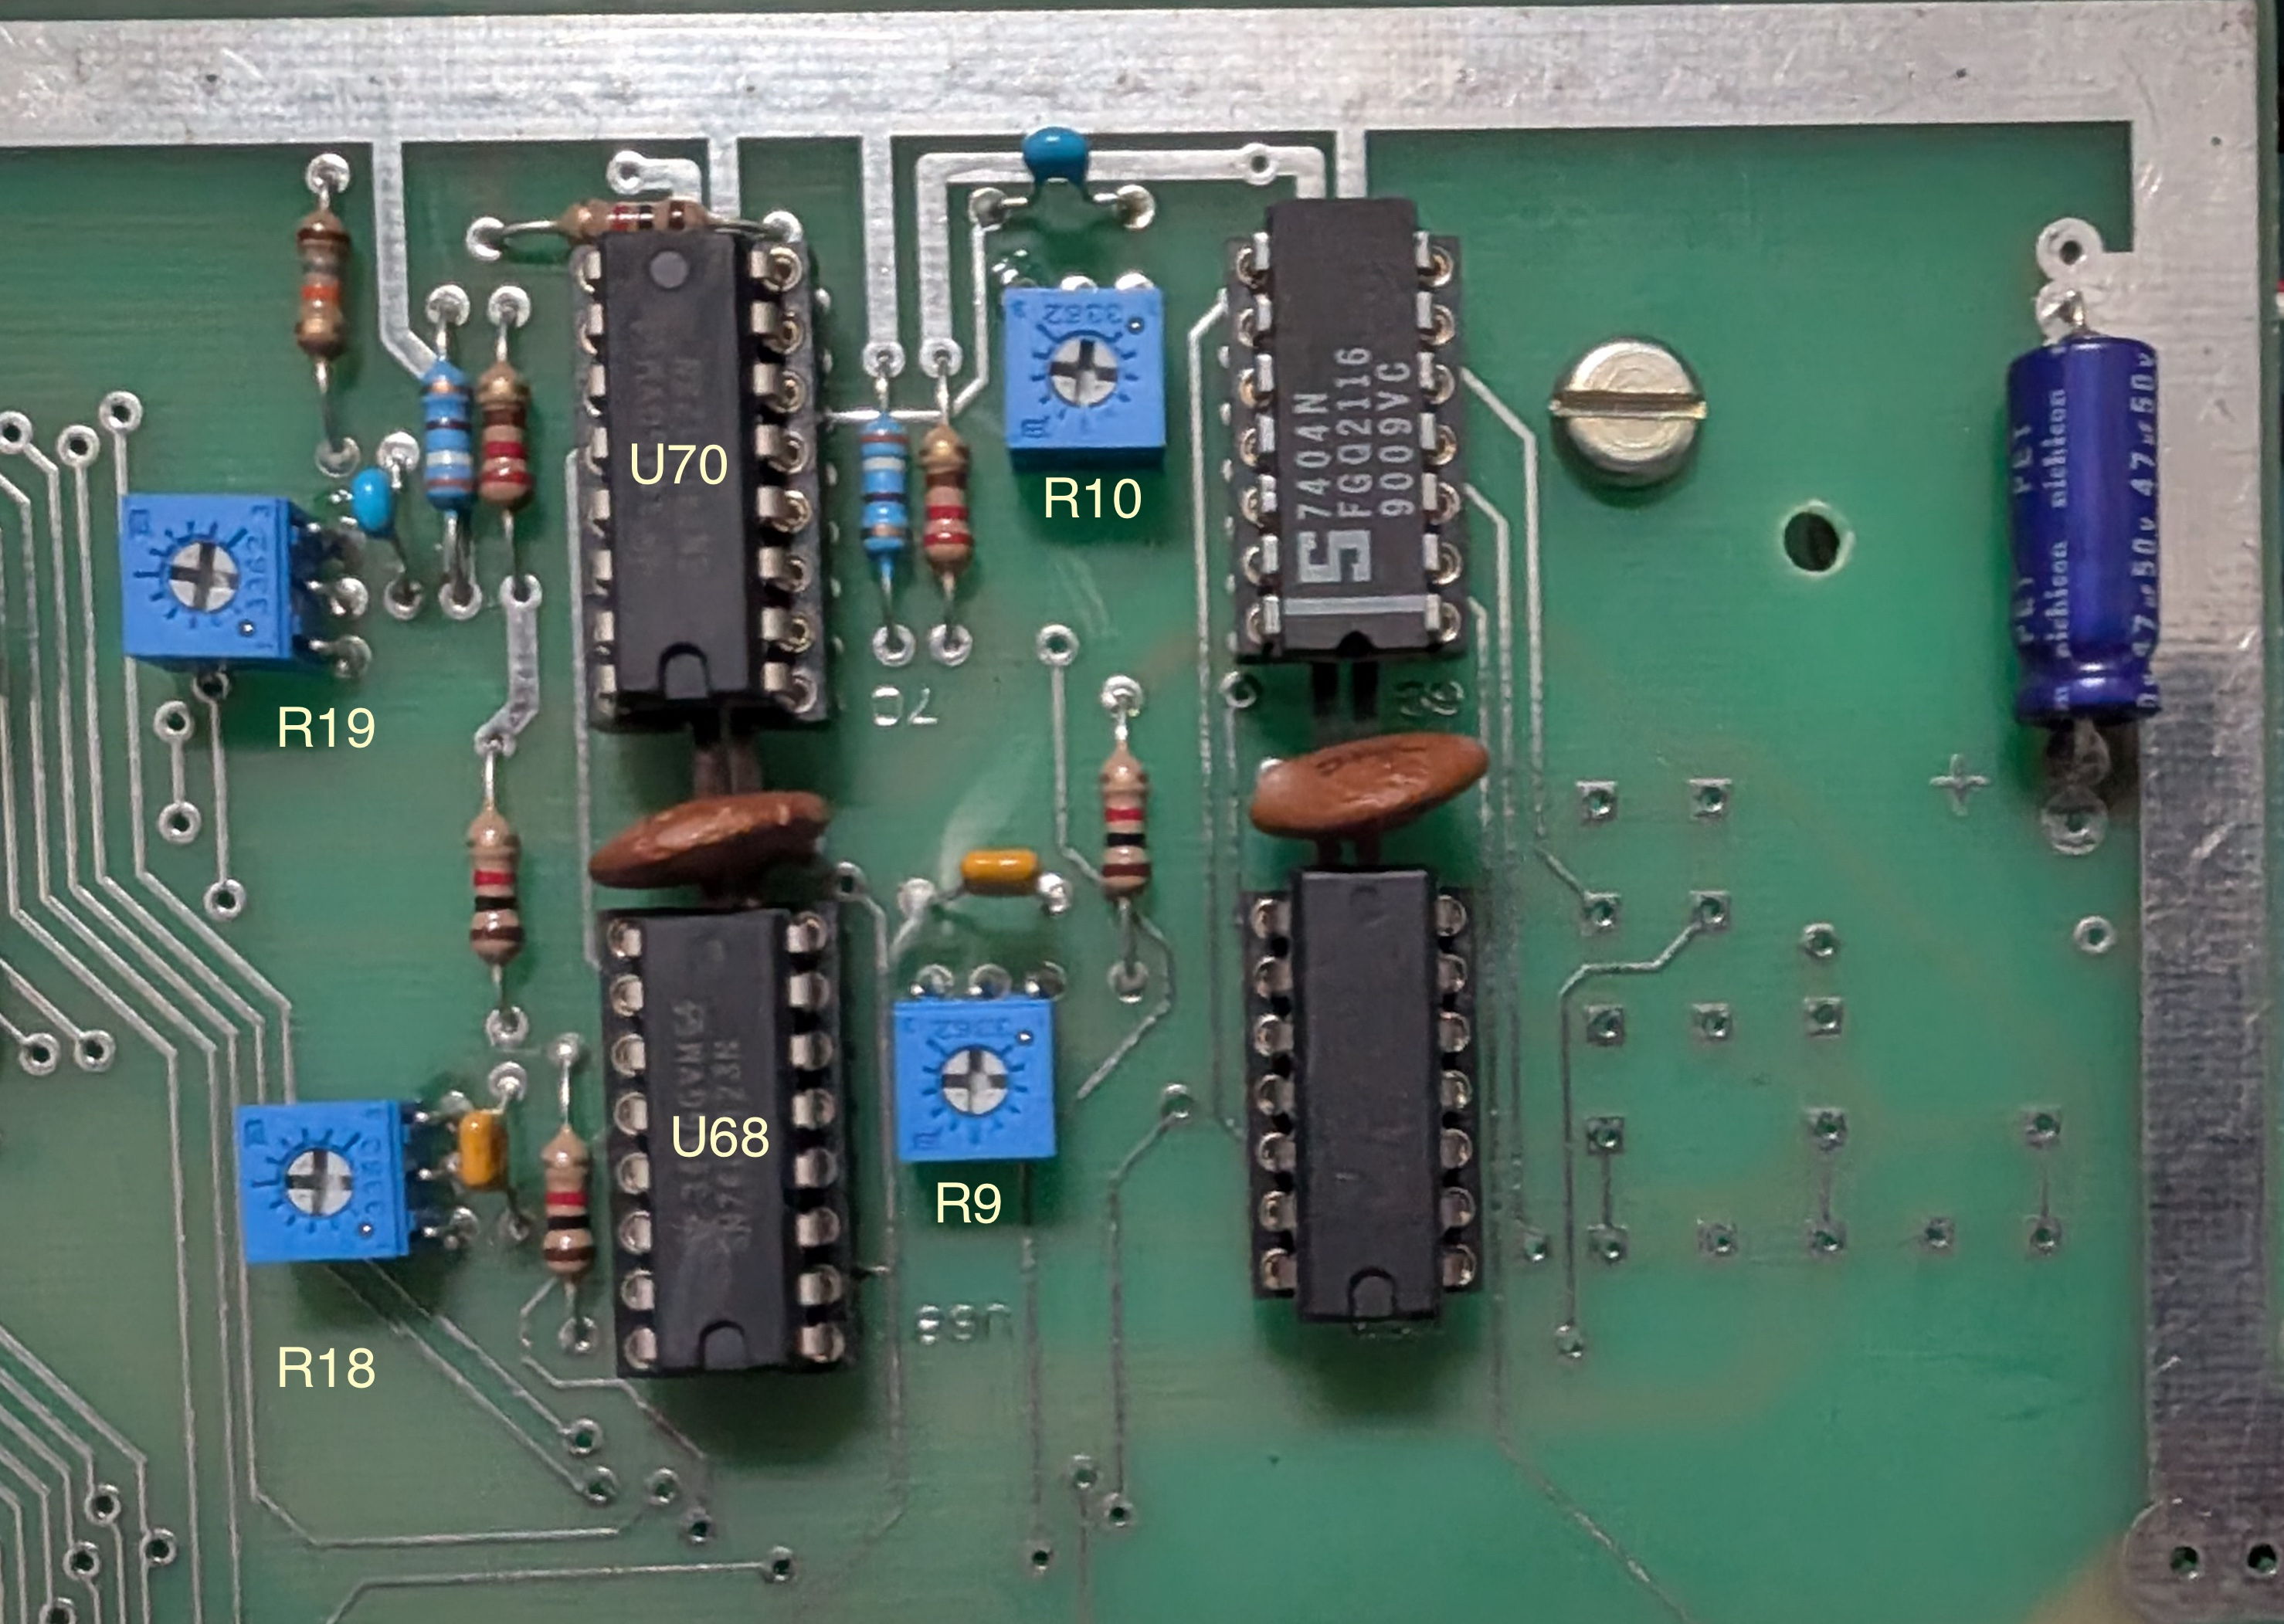
\includegraphics[width=4.9in]{images/U68-70.jpg}
\caption{Location of potentiometers.}
\label{fig:U68-70}
\end{center}
\end{figure}

\subsection{R18 TX CLOCK}

Input of scope to pin 13 of U68. Adjust R18 for a positive pulse width of 400nSec +/- 50nS. See \textbf{Fig. \ref{fig:R18}}.


\begin{figure}[htbp]
\begin{center}
\includegraphics[width=4.9in]{images/U68-13.png}
\caption{Adjusting R18.}
\label{fig:R18}
\end{center}
\end{figure}

\subsection{R9 TX DATA}

Input of scope to pin 12 of U68. Adjust R9 for a negative pulse width of 400nSec +/- 50nS. See \textbf{Fig. \ref{fig:R9}}.

\begin{figure}[htbp]
\begin{center}
\includegraphics[width=4.9in]{images/U68-12.png}
\caption{Adjusting R9.}
\label{fig:R9}
\end{center}
\end{figure}

\subsection{R10 RX CLOCK}

Connect a jumper from pin 9 of J3 to pin 10 of J3. Input of scope to pin 5 of U70, ee \textbf{Fig. \ref{fig:jumper}}.. Adjust R10 for a positive pulse width of 1uS. See \textbf{Fig. \ref{fig:R10}}.

\begin{figure}[htbp]
\begin{center}
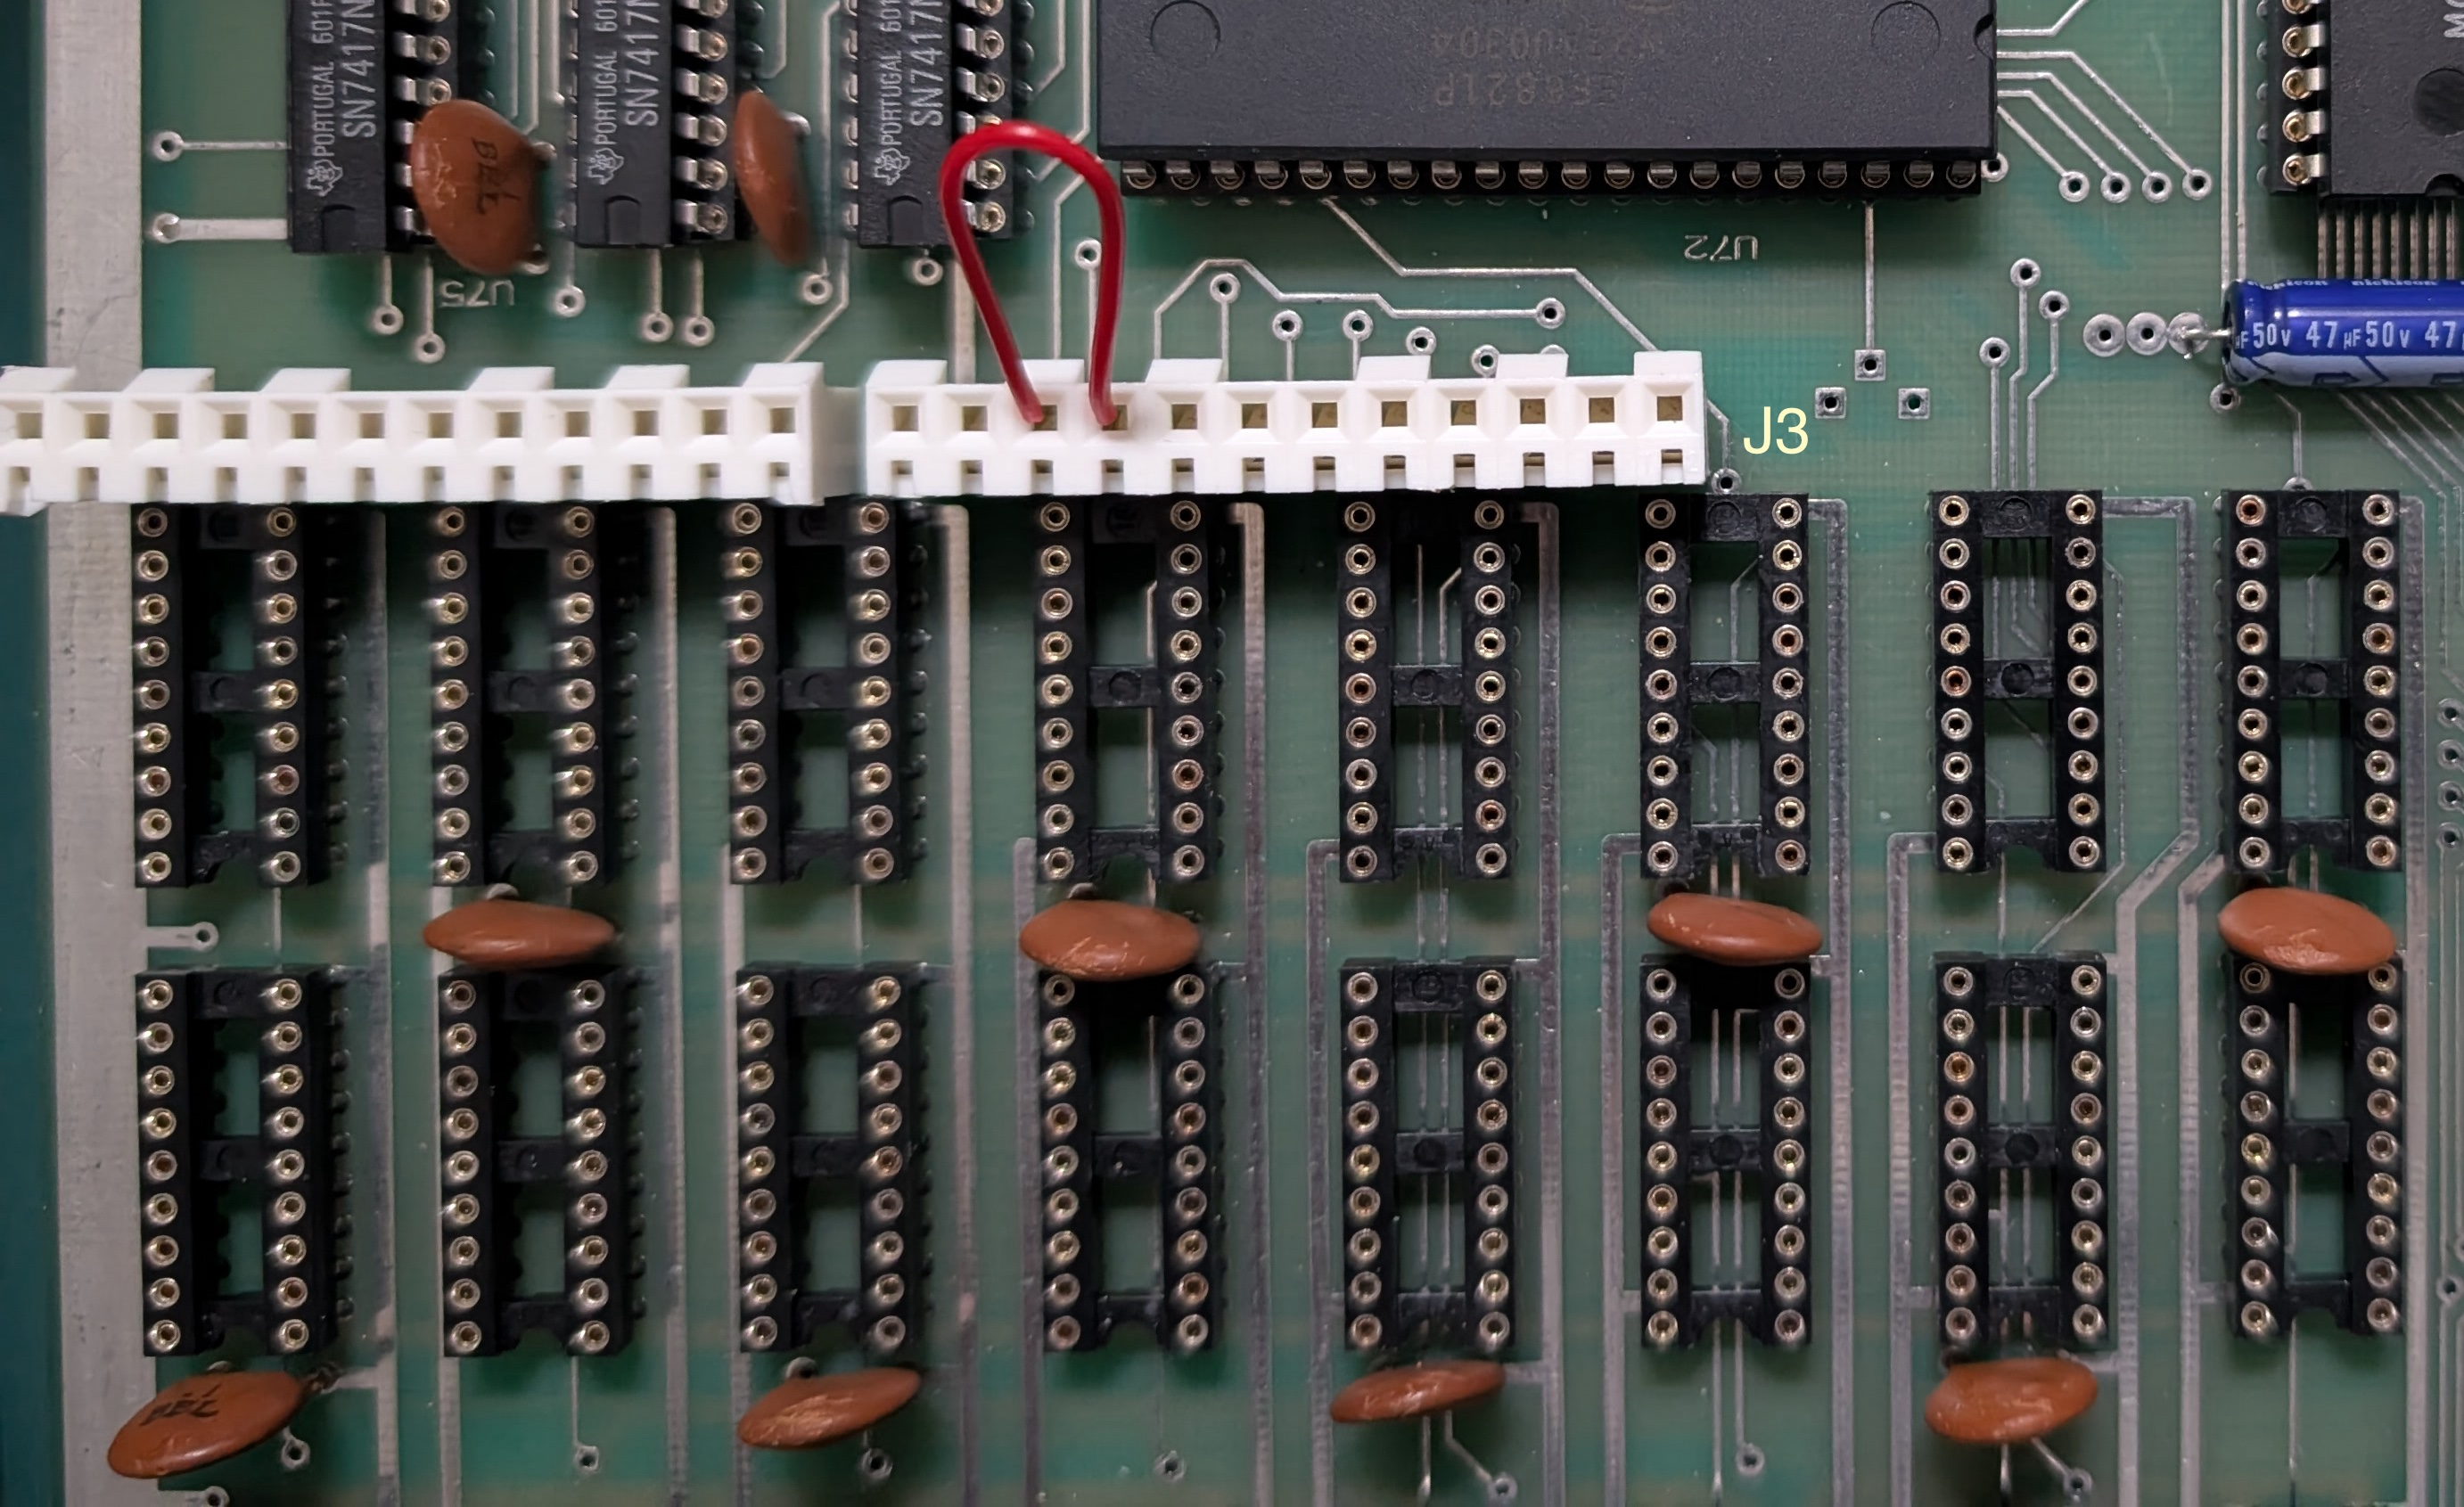
\includegraphics[width=4.9in]{images/9-10.jpg}
\caption{Jumper on J3, 9 to 10..}
\label{fig:jumper}
\end{center}
\end{figure}

\begin{figure}[htbp]
\begin{center}
\includegraphics[width=4.9in]{images/U70-5.png}
\caption{Adjusting R10.}
\label{fig:R10}
\end{center}
\end{figure}

\subsection{R19 RX DATA}

Connect a jumper from pin 9 of J3 to pin 11 of J3. Input of scope to pin 4 of U70 see \textbf{Fig. \ref{fig:R19}}. Adjust R19 for a negative pulse width of 6uS. Remove jumper and reconnect J3. See \textbf{Fig. \ref{fig:R19}}.

Some experiment with R20 (18k) may be required to obtain the correct pulse width. A value of 10k may be more appropriate.

\begin{figure}[htbp]
\begin{center}
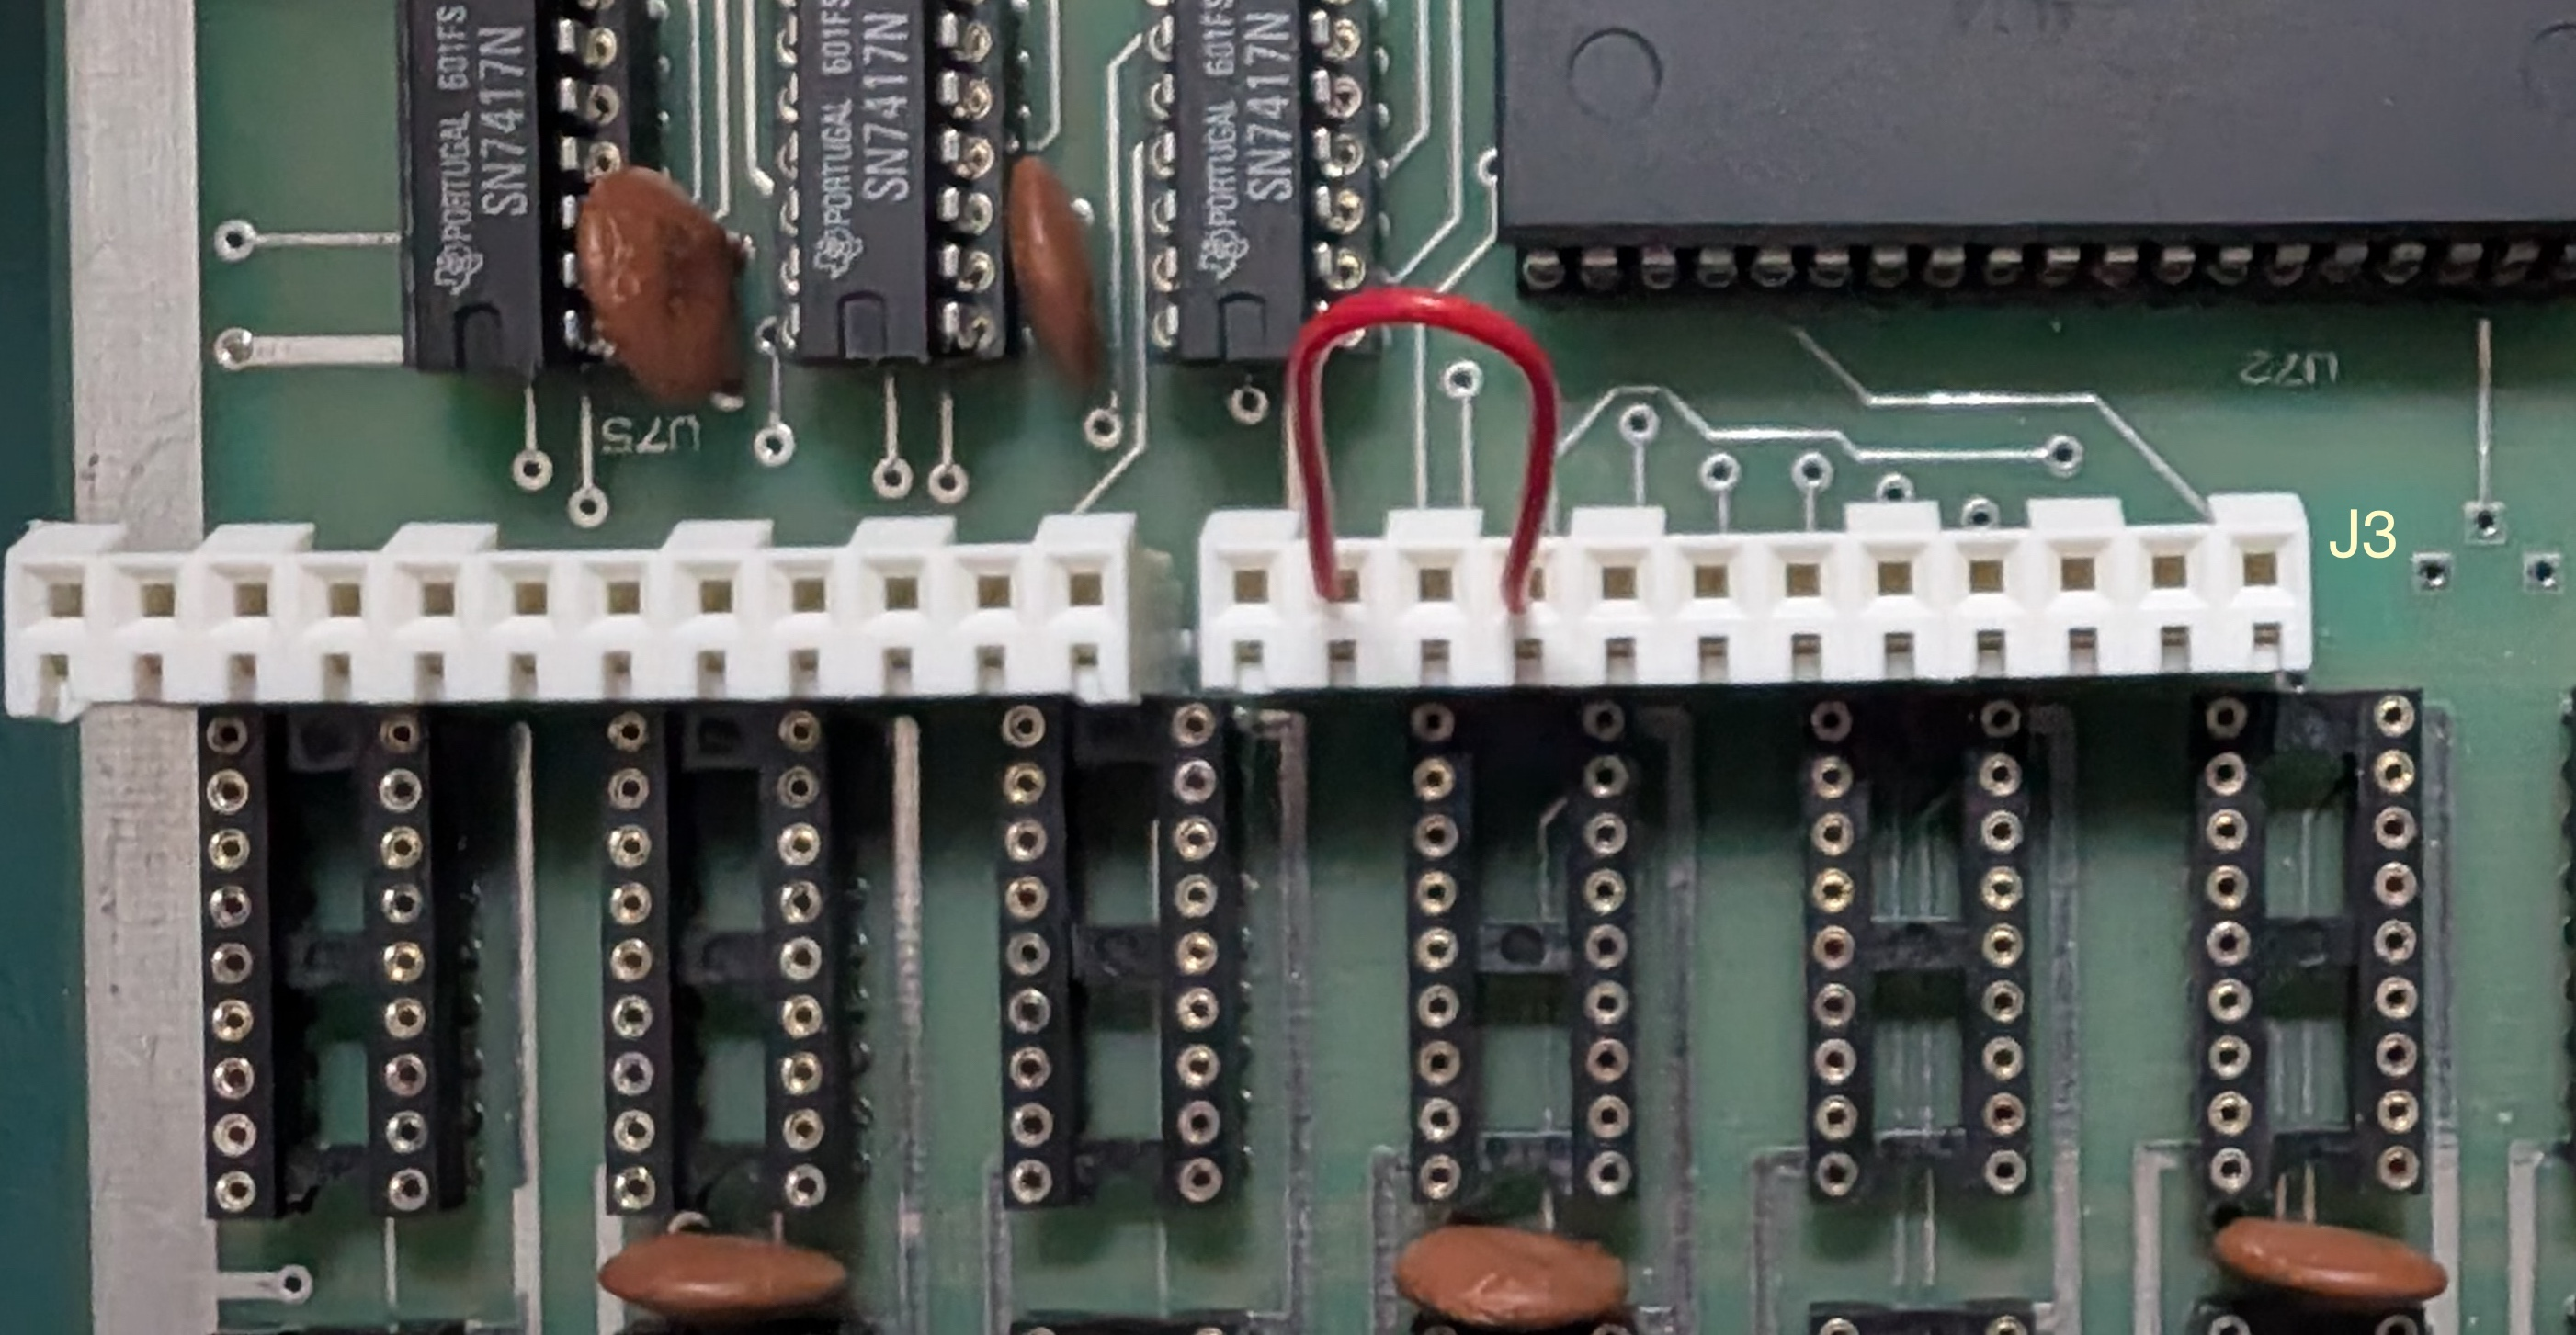
\includegraphics[width=4.9in]{images/9-11.jpg}
\caption{Jumper on J3, 9 to 11.}
\label{fig:jumper2}
\end{center}
\end{figure}

\begin{figure}[htbp]
\begin{center}
\includegraphics[width=4.9in]{images/U70-4.png}
\caption{Adjusting R9.}
\label{fig:R19}
\end{center}
\end{figure}



\section{D13 Data Separator Board}

With the board fitted, temporarily connect pin 9 of the 24 pin connector to link pin 1, see \textbf{Fig. \ref{fig:calibration-1}}. With the system powered up and no drives connected, set the input of the scope to pin 1 of IC4 and adjust R41 for a negative width of 6us. See \textbf{Fig. \ref{fig:calibration-2}}.

\begin{figure}[htbp]
\begin{center}
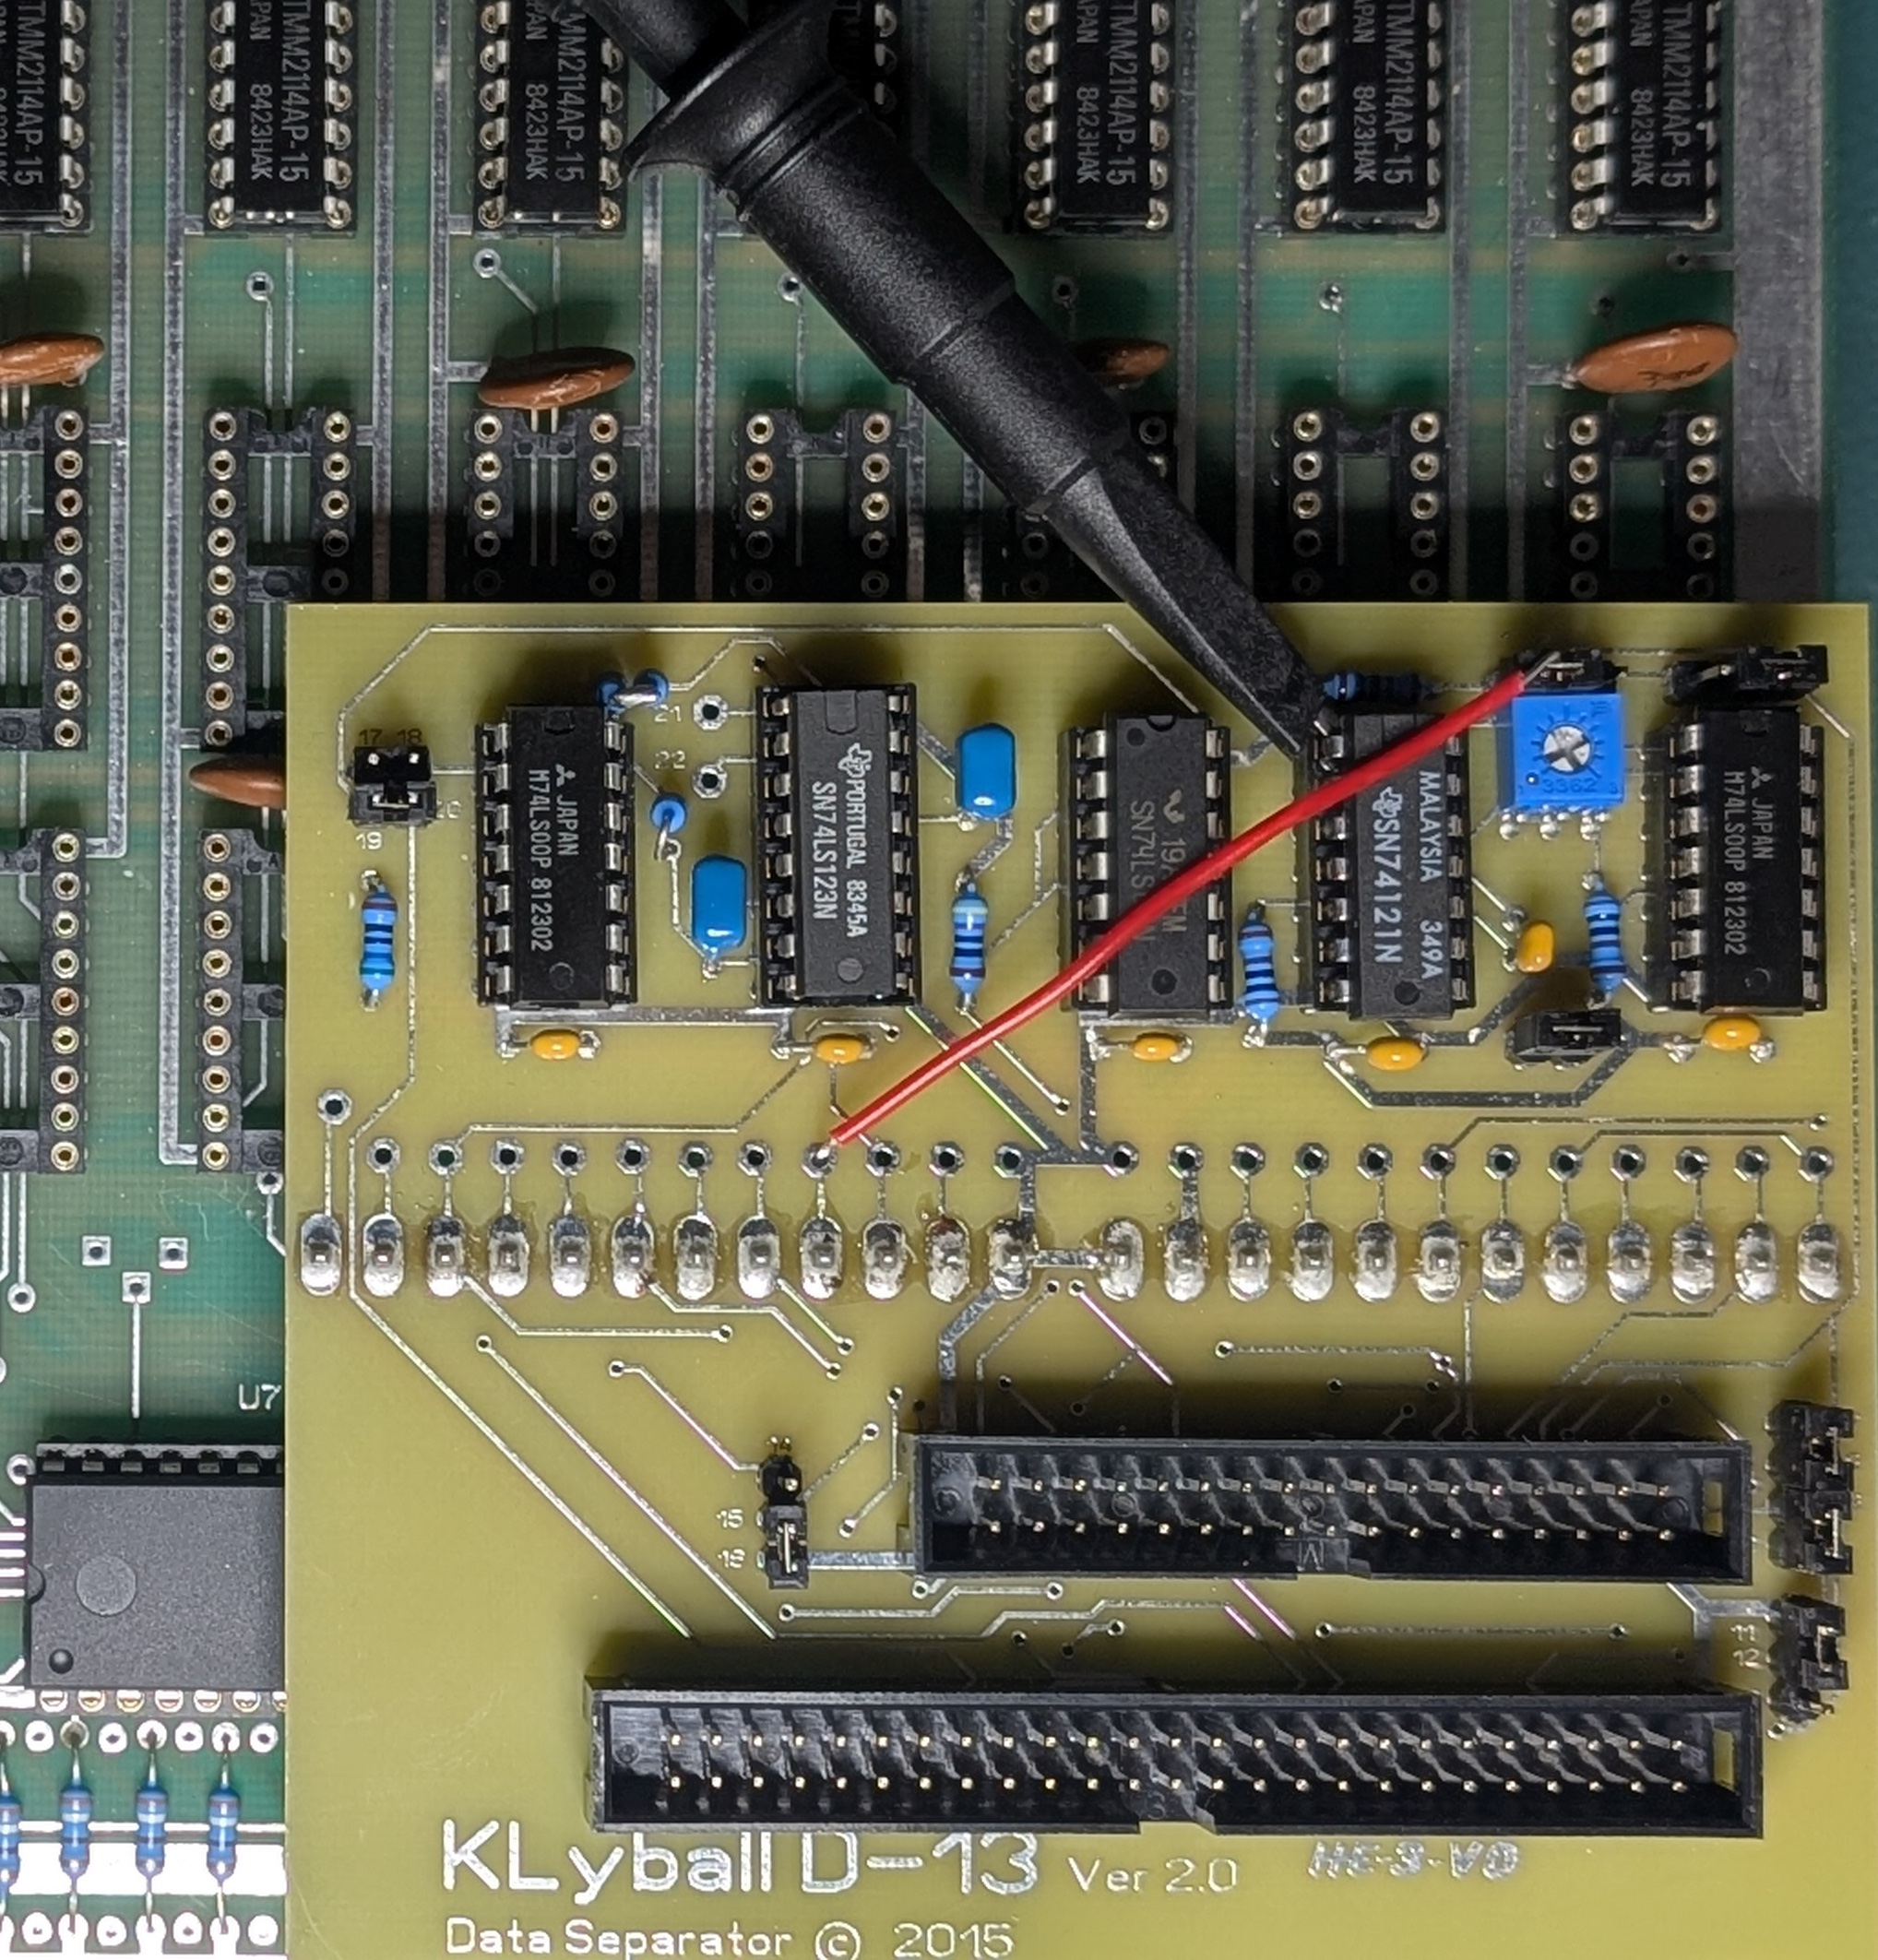
\includegraphics[width=4.9in]{images/Calibration-1.jpg}
\caption{Temporary link.}
\label{fig:calibration-1}
\end{center}
\end{figure}


\begin{figure}[htbp]
\begin{center}
\includegraphics[width=4.9in]{images/Calibration-2.png}
\caption{Adjusting R41.}
\label{fig:calibration-2}
\end{center}
\end{figure}

\section{Link Settings}

Please note that the links indicated on the schematic (see Appendices) are numbered differently to those on the board. Below is a table mapping the schematic diagram labels to the markings on the board itself.

\begin{BVerbatim}
    Board Link      Schematic Link
    ----------      --------------

    Pin 1           JP30    Pin 3
    Pin 2                   Pin 2
    Pin 3                   Pin 1
        
    Pin 4           JP33    Pin 1        
    Pin 5                   Pin 2
    Pin 6                   Pin 3
        
    Pin 7           JP35    Pin 4
    Pin 8                   Pin 3
    Pin 9                   Pin 2
    Pin 10                  Pin 1
        
    Pin 11          JP 34   Pin 1
    Pin 12                  Pin 2
    Pin 13                  Pin 3
        
    Pin 14          JP 1    Pin 3
    Pin 15                  Pin 2
    Pin 16                  Pin 1
        
    Pin 17          JP 2    Pin 2
    Pin 18                  Pin 4
    Pin 19                  Pin 1
    Pin 20                  Pin 3  
\end{BVerbatim}
        
The following link (placed between IC4 and IC6) is not marked on the board.

\begin{BVerbatim}
    a               JP 32   Pin 2
    b                       Pin 1
\end{BVerbatim}
        
The following link settings have been shown to work with both a C1/SBII with 610 and a 5.25 inch drive, and a C2 with D\&N board and a 5.25 inch drive.

Suggested links for 5.25 inch drives are shown below and in \textbf{Fig. \ref{fig:links}}. 

\begin{BVerbatim}
    1-2
    5-6
    a-b (unmarked link placed between IC4 and IC6, see above)
    7-8
    9-10
    11-12
    15-16
    19-20
\end{BVerbatim}

\begin{figure}[htbp]
\begin{center}
\includegraphics[width=4.9in]{images/LinkSettings.jpg}
\caption{Link Settings.}
\label{fig:links}
\end{center}
\end{figure}

\section{Checking the board}

With the Gotek attached, and a disk selected attach channel 1 of scope to the separated clock (pin 10 of the 24 way connector) and channel 2 to the separated data (pin 11 of the 24 way connector), and trigger the scope from channel 1. The data and clock signals should be clearly separated, see \textbf{Fig. \ref{fig:separation}}.

\begin{figure}[htbp]
\begin{center}
\includegraphics[width=4.9in]{images/data_separation.png}
\caption{Separated signals. Clock shown yellow and data shown blue.}
\label{fig:separation}
\end{center}
\end{figure}




